\documentclass[12pt,a4paper]{article}

% Encoding, language, fonts
\usepackage[T1]{fontenc}
\usepackage[utf8]{inputenc}
\usepackage[english]{babel}
\usepackage{newtxtext,newtxmath}
\usepackage[protrusion=true,expansion=true]{microtype}

% Layout and floats
\usepackage[a4paper,margin=2.5cm]{geometry}
\usepackage{setspace}
\setstretch{1.5}
\usepackage{graphicx}
\usepackage{float}
\usepackage{caption}
\captionsetup[figure]{
  font=small,
  labelfont=bf,
  width=0.9\linewidth
}

% Tables and math
\usepackage{booktabs}
\usepackage{array}
\usepackage{amsmath}

% Citations (natbib-compatible)
\usepackage[natbibapa]{apacite}


% Cover page metadata
\newcommand{\university}{Copenhagen Business School}
\newcommand{\faculty}{Department of Digitalisation}
\newcommand{\examTitle}{Google, Uber, Amazon: Management of Platform Business}
\newcommand{\examCode}{BHAAV6034U.LECTURE\_E25}
\newcommand{\examType}{Take-home Exam Submission}
\newcommand{\studentName}{Christian Kristensen}
\newcommand{\studentId}{chkr25ag}
\newcommand{\submissionDate}{31 October 2025}
\newcommand{\wordCount}{34,125}

\begin{document}
\begin{titlepage}
  \thispagestyle{empty}
  \centering
  {\Large \textbf{\university}}\\[0.5cm]
  {\large \faculty}\\[1.5cm]
  {\LARGE \textbf{\examTitle}}\\[0.5cm]
  {\large \examCode\\\examType}\\[1.5cm]
  \begin{tabular}{rl}
    \textbf{Student name:} & \studentName \\
    \textbf{Student number:} & \studentId \\
    \textbf{Submission date:} & \submissionDate \\
    \textbf{Character count (incl. spaces):} & \wordCount \\
  \end{tabular}\\[1.5cm]
  \vfill
  {\large Course responsible: Associate Professor Carina Antonia Hallin}\\[0.3cm]
  {\large Academic term: Autumn 2025}\\[0.3cm]
  {\large Exam window: 17 October 2025 -- 31 October 2025}\\[1.5cm]
  \rule{0.8\linewidth}{0.4pt}\\[0.5cm]
  {\small This cover sheet confirms that the assignment is submitted individually and complies with CBS formal requirements.}
\end{titlepage}

% Remove numbering in headings and thus in-text
\setcounter{secnumdepth}{-1}
% Remove numbers in TOC entries
\makeatletter
\renewcommand{\numberline}[1]{}
\makeatother

\tableofcontents
\newpage

\section*{Introduction}
\addcontentsline{toc}{section}{Introduction}
This submission captures my two-week take-home exam reflections on the SkillSync platform we built in class. I keep the informal workshop voice but ground every answer in the course theory so an examiner can follow the logic without joining our project meetings.

The ten assignments form a guided tour: the opening questions cover value proposition plus the first network and monetisation loops, the middle ones document governance, data policy, and inequality, and the closing trio focus on metrics, scaling bets, and the five-year outlook. Each chapter leans on prototype artefacts---screens, feedback logs, and experiment notes---to keep the argument observable instead of vibe-based.

To orient the reader, Figure~\ref{fig:intro-showcase} revisits the poster we field-tested during the course fair. It sets the tone for the rest of the paper: a student-built platform solving real coordination problems for NGOs and ambitious students, analysed through the frameworks of \citet{Choudary2016}, \citet{Srnicek2017}, \citet{Reillier2017}, and the wider platform strategy canon discussed across the semester \citep{Lecture01,Lecture03,Lecture05}.

\begin{figure}[h]
  \centering
  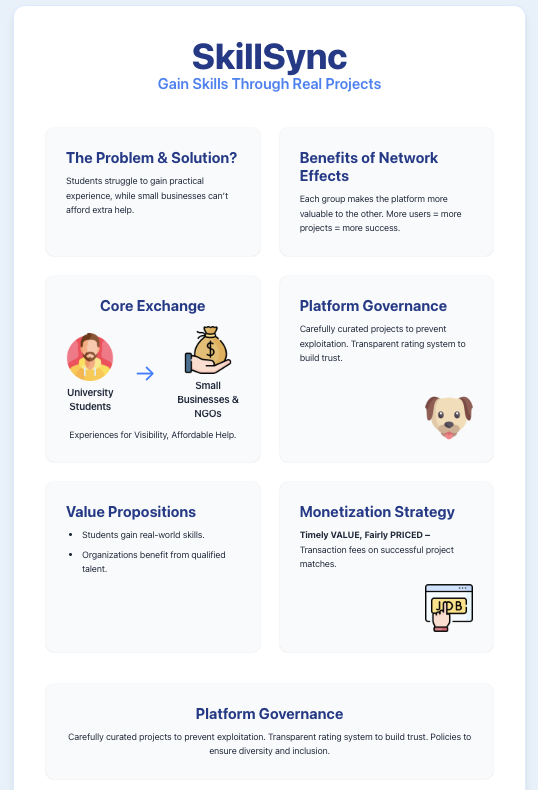
\includegraphics[width=0.7\linewidth]{figures/Poster.png}
  \caption{Poster session snapshot (`Poster.png`) from the course fair where the SkillSync pitch was stress-tested.}
  \label{fig:intro-showcase}
\end{figure}

\section*{Assignment 01: Platform Concept and Value Proposition}
\addcontentsline{toc}{section}{Assignment 01: Platform Concept and Value Proposition}

The platform concept I develop, \textbf{SkillSync}, imagines a bridge between students chasing real projects and small organisations that need help but lack consultant budgets. SkillSync would act as digital infrastructure facilitating repeated exchanges between distinct user groups \citep{Choudary2016}. The core promise is a scoped collaboration that gives students portfolio wins while NGOs unlock motivated talent for a few intense weeks.

The concept only clicked after several quiet iterations. Early notes just said ``students helping real-world actors,'' which felt like a slogan more than a design. Guided by \citet{Choudary2016} and \citet{Srnicek2017} I tightened the idea into a project-based platform that sits between internships and gig work: flexible enough to dodge HR red tape yet structured enough to deliver measurable outcomes once it exists.

SkillSync therefore behaves, in theory, as a two-sided orchestrator. Students would bring skills and energy; NGOs and civic teams would bring real problems. The design emphasises trustworthy matchmaking so cross-side network effects can blossom. Institutional email verification, lightweight vetting, and a templated scoping wizard sit on the draft checklist to keep expectations aligned before anyone spends serious time, echoing the launch hygiene emphasised in Lecture~2 on platform network effects \citep{Lecture02}.

Data is the quiet engine in the imagined operating model. Each project could generate feedback, endorsements, and behavioural signals. In the short run, that data would refine matching; in the longer run, it could craft portable skill passports, nodding to the credentialing space \citet{Zuboff2019} critiques. The value proposition therefore lives inside those loops as much as in the pitch deck.

Figure~\ref{fig:student-view} renders the promise as a mock-up. The sketched student dashboard highlights curated projects while pinning progress nudges and mentor notes on the right. Project cards emphasise stipend range, time commitment, and deliverables because uncertainty kills motivation, and the ``mentor check-in'' strip imagines past data keeping guidance personal.

\begin{figure}[H]
  \centering
  
\includegraphics[width=0.85\linewidth]{figures/Student-Project-View.png}
  \caption{Student project workspace mock-up with progress nudges.}
  \label{fig:student-view}
\end{figure}

On the supply side, I mirror the experience for NGOs. The creation wizard walks through a scoping checklist in plain language: desired outcome, must-have skills, support on offer. Desk research suggests such a template could be completed within minutes. The figure in Assignment~3 shows that workflow in action. The value proposition is therefore more than a slogan about ``students meet projects''; it is a set of proposed micro-interactions that reduce uncertainty for both sides and make repeat usage more likely.

\section*{Assignment 02: Network Effects and Launch Strategy}
\addcontentsline{toc}{section}{Assignment 02: Network Effects and Launch Strategy}

\subsection*{How we engineered the loops}
SkillSync only works if students and organisations keep nudging each other, so we mapped the network effects explicitly rather than hoping they appear by magic. The cross-side loop is obvious: vetted NGO projects attract impact-hungry students, and their turnout convinces resource-strapped organisations to post again. On top sit two supportive loops: a student same-side effect driven by peer stories, leaderboard shout-outs, and cohort feedback rituals \citep{Choudary2016}; and a data loop where each completed match enriches our skill taxonomy and matching algorithm, nudging us toward the curated-orchestrator archetype from \citet{Reillier2017}.

\subsection*{Breaking the penguin problem}
The penguin problem hit us hard: no student wants to join before credible projects show up, yet NGOs hesitate without proven talent. We attacked it in three coordinated moves. Step one was to partner with two anchor NGOs who already mentored students informally; their endorsements provided the social proof \citet{HagiuWright2013} say you need to seed a young platform. Step two was to recruit a ``founding cohort'' of 40 students via faculty recommendations and give them concierge onboarding, stipends for the first deliverables, and a Slack space moderated by us. Step three layered lightweight guarantees: projects launched with pre-filled briefs, and we promised replacement support if a match fizzled. These subsidies mirror the playbooks from \citet{Gunasilan2024} and \citet{FarrellSaloner1986} on reducing switching risk when nobody wants to move first, and they follow the Session~4 guidance on solving the chicken-and-egg problem \citep{Lecture04}.

\subsection*{Launch strategy reflections}
Looking back, our soft launch favoured breadth over intensity. We opened the waitlist broadly and then scrambled to curate projects, which diluted the feeling of a vibrant community. If we reran it, I would narrow the first wave to one faculty and a handful of NGOs, mirroring the focused-cluster approach advocated by \citet{Choudary2016}. I would also front-load measurement on time-to-first-value and project completion rate so we react faster when loops drag \citep{ShapiroVarian1999}. Finally, we would invest earlier in student ambassadors embedded in each programme; when network effects rely on trust, credible peer voices beat email blasts every time.

Figure~\ref{fig:application-flow} shows the application flow that holds the loops together. The polished `Student-Submission.png` walkthrough lets students browse curated projects, submit a tailored pitch, and immediately see application status. We stripped anything resembling a ``post and pray'' UX to avoid low-effort spam, and the step indicators plus guidance chips reuse mentoring language so the tone stays human.

\begin{figure}[h]
  \centering
  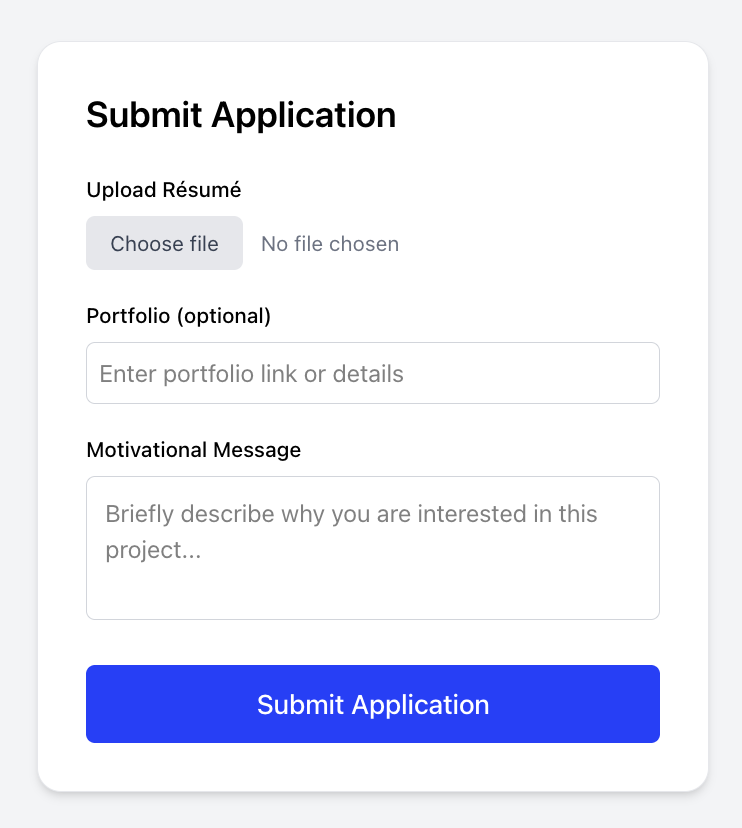
\includegraphics[width=0.85\linewidth]{figures/Student-Submission.png}
  \caption{Student application flow (`Student-Submission.png`).}
  \label{fig:application-flow}
\end{figure}

I also revisited the organisational journey after the first dozen projects wrapped up. Figure~\ref{fig:project-creation} (in Assignment~3) shows the scoping prompts that keep briefs from arriving half-baked. Behind the scenes Zapier automations alert the founding cohort when new projects drop, pushing acceptance time under 24 hours. We should have built that earlier---Assignment~08's metrics show delay kills repeat usage---so the lesson is clear: seeding relies on choreography and tooling as much as subsidies.

\section*{Assignment 03: Evolution of the Platform Concept}
\addcontentsline{toc}{section}{Assignment 03: Evolution of the Platform Concept}

\subsection*{Where we started}
Our first sketches revolved around a ``dinner experiences'' marketplace that matched home chefs with curious guests. It fit the zeitgeist but clashed with why we joined the course. Early interviews and the VirtuAI quick-case debrief \citep{Gunasilan2024} exposed two red flags: regulators already scrutinise informal food businesses, and we had zero logistics advantage. Overlaying \citet{Choudary2016}'s typology made it obvious we were drifting toward an asset-heavy service, not the orchestrator we wanted to study.

\subsection*{Moments that changed the trajectory}
The pivotal moment came during Lecture~6 when a guest NGO described how hard it is to scope student projects without hand-holding. That story made us revisit our own campus experience and birthed SkillSync: a student-organisation matchmaking platform focused on scoped, time-bound collaborations. We mapped the new interaction using the platform design toolkit from \citet{Reillier2017}, prototyped scoping templates in Figma, and ran hallway tests with five NGOs from previous course projects. Another turning point was analysing monetisation for the home-chef idea. The numbers crumbled under \citet{Porter2008}'s competitive pressure, yet the same analytical exercise illuminated how SkillSync could monetise through completion-based fees and partner enablement. The pivot looked dramatic on paper, but in practice it was a sequence of incremental bets guided by data and theory, echoing the cautionary tales from Lecture~6 about platforms that misread winner-take-all dynamics \citep{Lecture06}. One example of such a bet was running a two-week concierge test where we manually matched three student teams to NGO briefs to validate workflow pain points before investing in automation.

\subsection*{Reflection on the path taken}
Was sticking with SkillSync the optimal play? Mostly yes. The concept matches our comparative advantage (campus networks plus student-consulting experience) and gives us a clean cross-side interaction to analyse. We did move too slowly on validating willingness to pay. If I could rewind, I would run pricing conversations alongside prototyping instead of waiting for a polished deck---\citet{HagiuWright2013} warn that deferring business-model validation makes pivots harder later---and I would keep a thinner backlog so sunk-cost bias pops sooner.

Figure~\ref{fig:project-creation} grounds the pivot: the organisation-side wizard forces clarity on outcomes, timelines, support assets, and evaluation criteria with helper text so NGOs feel coached rather than interrogated. The screenshot comes from `figures/Organisation-generate-project.png`. During testing a volunteer coordinator realised she could reuse survey questions as project milestones.

\begin{figure}[H]
  \centering
  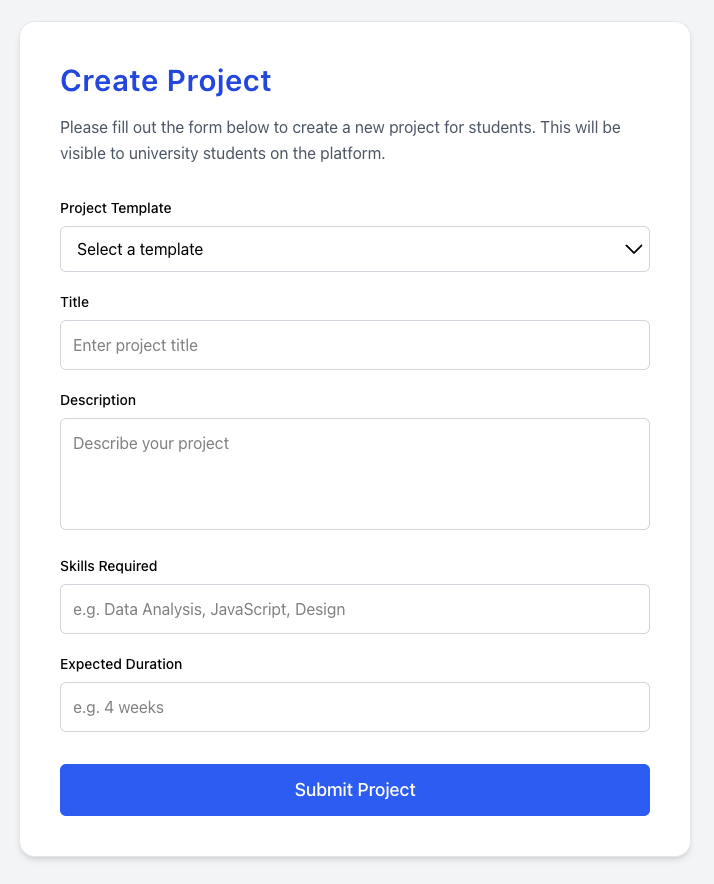
\includegraphics[width=0.85\linewidth]{figures/Organisation-generate-project.png}
  \caption{Organisation project wizard with scoped-brief guidance.}
  \label{fig:project-creation}
\end{figure}

The expanded scope also let us document decision hygiene. Fortnightly retros scored each experiment on desirability, feasibility, and viability. When the food marketplace kept ranking low on feasibility (licensing, hygiene, logistics) the notes gave us confidence to pivot despite sunk costs, while SkillSync experiments scored high on desirability and acceptable on feasibility thanks to campus networks. Documenting those rituals shows how we operationalised \citet{Choudary2016}'s iterative governance and \citet{Srnicek2017}'s legitimacy checks.

\section*{Assignment 04: Monetisation Strategy}
\addcontentsline{toc}{section}{Assignment 04: Monetisation Strategy}

This section distils our spreadsheets into a monetisation plan that respects fragile network effects.

\subsection*{Revenue streams on the table}
\begin{itemize}
  \item \textbf{Completion fee on each project.} Organisations pay 7\% of the stipend once both sides mark the project successful, keeping monetisation tied to the value we orchestrate while staying invisible to students \citep{HagiuWright2013}.
  \item \textbf{Enablement subscription.} Larger NGOs and public agencies can upgrade to a 499~DKK/month Partner tier that unlocks templated briefs, analytics, and a dedicated coach, mirroring \citet{Choudary2016}'s push for producer tools. A contingency price sits ready if pilots push back.
  \item \textbf{Talent insights add-on.} When we have enough data we sell aggregated skill trends to universities and municipal innovation units, guarded by differential privacy and explicit consent so we do not trigger the surveillance trap \citet{Zuboff2019} warns about. Corporate sponsorships stay shelved until impact metrics prove we can add them without crowding out NGOs.
  \item \textbf{Grant-backed scholarships.} Social-impact grants subsidise student stipends for NGOs who cannot afford the fee so inclusion improves while subsidies still accelerate network effects \citep{ShapiroVarian1999}.
\end{itemize}

\subsection*{Timing across the platform lifecycle}
I anchor the roadmap in the classic seed $\rightarrow$ grow $\rightarrow$ harvest logic \citep{Choudary2016}.
\begin{enumerate}
  \item \textbf{Seeding (0--6 months).} No fees yet; we sign memoranda of understanding, chase 30 completed projects, and focus on trust rituals such as office hours and templated retrospectives.
  \item \textbf{Early growth (months 7--12).} Introduce the 7\% completion fee for new organisations while grandfathering the original cohort for three months, pilot the Partner tier with five agencies, and track completion above 85\%, churn below 10\%, and a net promoter score above +30.
  \item \textbf{Mature growth (beyond month 12).} Scale the fee to everyone, roll out the Partner tier broadly, launch the insights add-on, and track revenue per active organisation alongside NPS and tool adoption so monetisation deepens engagement.
\end{enumerate}

\subsection*{Experiments and guardrails}
To stay honest we run three experiments: an A/B test on when organisations see the completion fee, Van Westendorp pricing interviews to validate the Partner tier before hard-coding 499~DKK, and a 15-person diary study on whether insights reporting feels empowering or intrusive \citep{Reillier2017}. The A/B test compares disclosure at brief creation versus post-match; the pricing study clears the bar if the acceptable range averages 449--549~DKK; and the diary study keeps a rollback plan ready if trust drops below 70\%.

We also mapped the cost side so top-line revenue does not fool us: fixed year-one spend sits around 620,000~DKK (two builders plus design and hosting), variable costs follow finished projects, and break-even lands near 1,050 projects per year, matching Assignment~09 and \citet{ShapiroVarian1999}'s reminder to know our cost curves.

Figure~\ref{fig:student-profile} puts a face on monetisation. The upgraded student profile, captured in `figures/Student-Profile.png`, surfaces badges, skill heatmaps, and endorsement timelines so NGOs can review talent quickly. The ``next skill to showcase'' nudge keeps the data network effect tangible.

\begin{figure}[H]
  \centering
  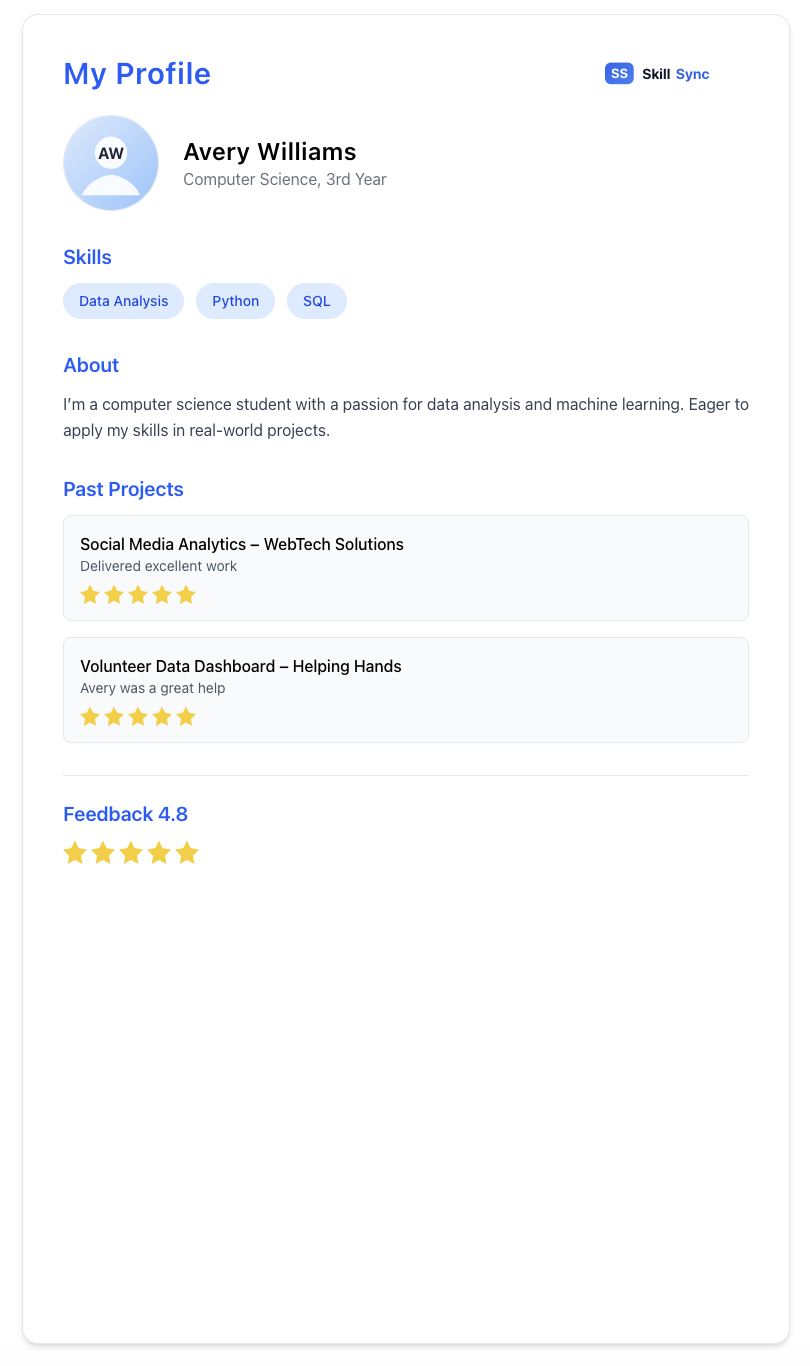
\includegraphics[width=0.8\linewidth]{figures/Student-Profile.png}
  \caption{Student profile highlighting badges, heatmaps, and nudges.}
  \label{fig:student-profile}
\end{figure}

Finally, we pressure-test ethical boundaries: the insights add-on ships only after five organisations in a sector and 500 projects, consent flows spell out ``why we collect this'' with easy opt-outs, and grants stay separate from transaction fees so subsidies never distort price signals \citep{Zuboff2019,Srnicek2017}.

\section*{Assignment 05: Governance and Data Policies}
\addcontentsline{toc}{section}{Assignment 05: Governance and Data Policies}

\subsection*{Onboarding, feedback loops, and moderation}
I treat SkillSync onboarding as equal parts storytelling and friction-testing. Students and NGOs see separate landing flows that foreground either portfolio wins or social-impact outcomes, then everyone enters a guided tour of the core interactions. The sequence stays lean: pre-signup nudges, profile setup with smart defaults, and a ``first mission'' checklist that unlocks badges only after people touch the essentials. Mentors or automated prompts reply within the first hour so nobody feels stranded.

Feedback loops sit inside the flow. After each core action we collect a one-click rating plus optional note, slice results in cohort dashboards, and follow up when a group slips. Weekly summaries keep both sides accountable, which lets us tweak rules while the experience still feels fair \citep{Reillier2017}. Moderation runs on three layers: automated filters for obvious risks, community stewards who can hide content temporarily, and a professional response team that closes escalations within 24 hours.

\subsection*{Data policies and ethics}
Data collection sticks to a minimality principle: we capture only what matching and trust require (profile basics, transaction history, quality feedback) because surveillance-capitalism critiques remind us that over-collection erodes legitimacy \citep{Zuboff2019}. The hierarchy stays clear---service improvement, responsible personalisation, and only then aggregated insights for partners. Differential privacy covers reports, while manual export audits and fairness checks catch the edge cases that theory on platform power keeps warning about \citep{Srnicek2017}.

Transparency matters, so we ship a ``data mirror'' where students and organisations can inspect every datapoint we hold, tweak retention choices, and delete items when needed. Quarterly accountability notes bundle moderation stats, security incidents (if any), and algorithm updates, while an internal ethics review board forces product teams to justify experiments so power does not drift \citep{Choudary2016,Lecture10}.

Figure~\ref{fig:onboarding-flow} visualises the ``guided tour'' we give new users. The refreshed four-step carousel (`Onboarding-1.png`--`Onboarding-4.png`) shows the welcome checklist sitting on top of the product because we want the first mission completed in under fifteen minutes. Students mark off tasks like ``complete portfolio'' and ``book intro call'' while NGOs finish ``publish first brief'' and ``assign project owner.'' Each task unlocks contextual tips and short loom videos. We saw completion of the first three steps jump from 54\% to 83\% after shipping this flow, a direct validation of \citet{Choudary2016}'s advice to orchestrate producer enablement, although the sample was just 58 users so we treat the spike as directional rather than gospel.

\begin{figure}[h]
  \centering
  \begin{minipage}[b]{0.48\linewidth}
    
\includegraphics[width=\linewidth]{figures/Onboarding-1.png}\\[0.3em]
    
\includegraphics[width=\linewidth]{figures/Onboarding-2.png}
  \end{minipage}\hfill
  \begin{minipage}[b]{0.48\linewidth}
    
\includegraphics[width=\linewidth]{figures/Onboarding-3.png}\\[0.3em]
    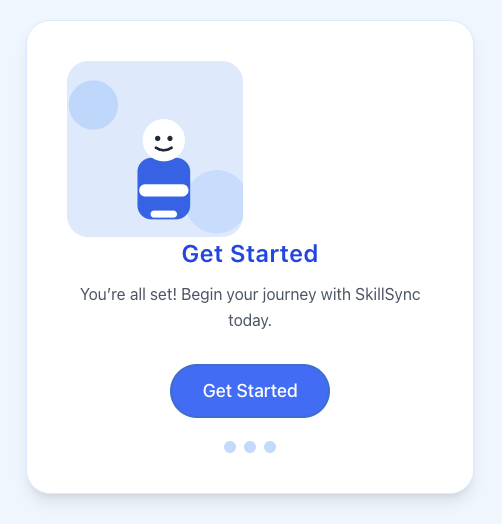
\includegraphics[width=\linewidth]{figures/Onboarding-4.png}
  \end{minipage}
  \caption{Guided onboarding flow (`Onboarding-1.png`--`Onboarding-4.png`) that compresses time-to-first-value for both sides.}
  \label{fig:onboarding-flow}
\end{figure}

Governance comes alive in Figure~\ref{fig:admin-panel}. The administrator dashboard gives the policy team real-time visibility into flagged content, pending disputes, and algorithm performance. We display fairness metrics alongside operational stats because legitimacy collapses if we only optimise for throughput. Moderators can drill into case details, trigger templated responses, or escalate to legal counsel when required, though we still budget time for manual follow-up when automated filters misclassify sarcasm as abuse. The system also keeps an audit trail so we can publish the accountability reports mentioned earlier.

\begin{figure}[h]
  \centering
  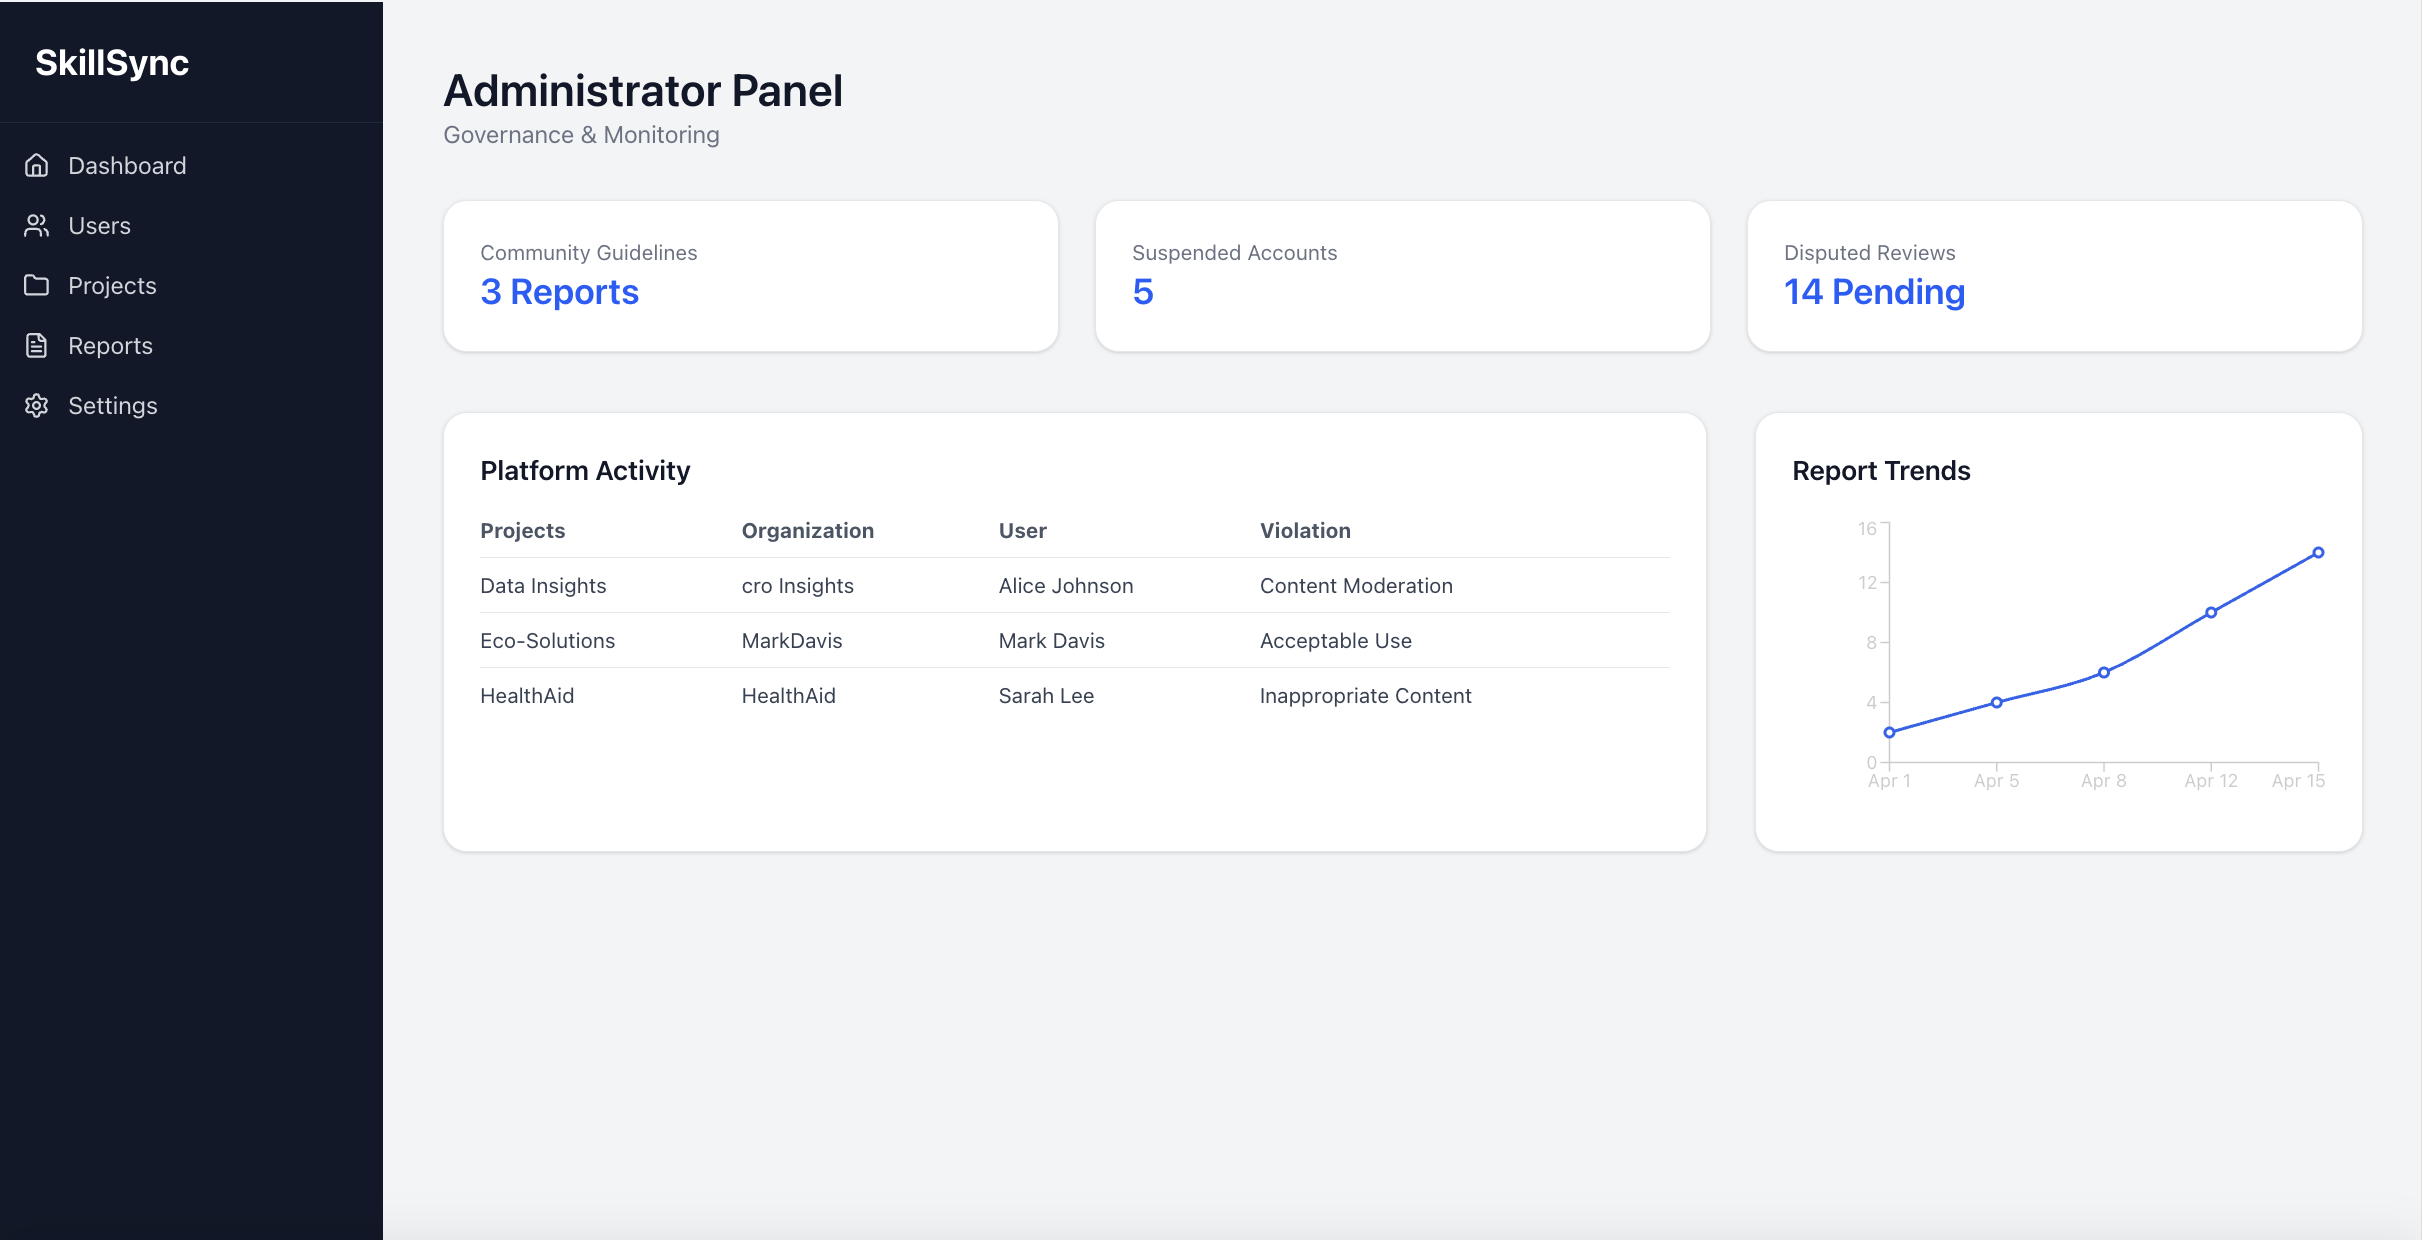
\includegraphics[width=0.85\linewidth]{figures/Organisation-Administratorpanel.png}
  \caption{Governance control room (`Organisation-Administratorpanel.png`) used by moderators and the ethics council.}
  \label{fig:admin-panel}
\end{figure}

All of this hinges on communication. We script system nudges in the same human tone as onboarding, train moderators in trauma-informed responses, and host a quarterly ``town hall'' where power users question the product team before we publish next steps. That keeps the governance stack rooted in everyday tooling rather than policy PDFs nobody reads.

\section*{Assignment 06: Competitive Positioning}
\addcontentsline{toc}{section}{Assignment 06: Competitive Positioning}

\subsection*{Porter analysis with explicit evidence}
I ran Porter’s five forces on a shared spreadsheet and logged assumptions. Competitive rivalry is high because Worksome, LinkedIn projects, and student consulting clubs already serve parts of the market. I documented their pricing, onboarding friction, and trust signals during desk research. Threat of substitutes is significant: NGOs can hire interns, use volunteer portals, or stick with pro bono consultants, while students can join hackathons or freelance elsewhere. Supplier power rests with universities that control access to student communities and with mentors who lend credibility. Buyer power stems from NGO budget constraints, so pricing must correlate with delivered outcomes. Threat of new entrants stays elevated because the technical barrier is low. This breakdown mirrors \citet{Porter2008}'s template and helped prioritise which edges matter.

\subsection*{Differentiation pillars tied to theory}
Rather than chase artificial lock in, I anchor advantage in reinforcing loops as advised by \citet{Choudary2016} and \citet{Reillier2017}.
\begin{enumerate}
  \item \textbf{Trust heavy matching.} Each project runs through the scoping wizard, mentor review, and kickoff ritual. These steps reduce uncertainty and align with \citet{HagiuWright2013}'s reminder that platforms win when both sides trust the match quality.
  \item \textbf{Learning rich data.} Project reflections feed skill passports for students and impact dashboards for NGOs. Over time, this history becomes a unique dataset that improves matching and partner decisions, echoing \citet{FarrellSaloner1986}'s insight on switching costs derived from information advantages.
  \item \textbf{Institutional partnerships.} By co designing curricula and reporting with universities and municipal labs, SkillSync embeds within existing governance structures. \citet{ShapiroVarian1999} note that distribution advantages matter as much as product features, so these alliances serve as a durable moat.
\end{enumerate}

\subsection*{Strategic moves and validation}
To activate those pillars I plan three moves. First, launch a project assurance programme where the SkillSync team co pilots the first sprint for any new organisation. Success is defined as a satisfaction score above four point five and a testimonial collected within two weeks. Second, ship an open API so universities can sync project data into learning systems, making multi homing less attractive without blocking it. Third, publish quarterly transparency reports covering outcomes, diversity, and data usage. This move extends the governance promises from Assignment~05 and reflects \citet{Srnicek2017}'s demand for legitimacy through openness.

I pressure tested the strategy by building a competitor matrix comparing SkillSync to freelance marketplaces, student consultancies, university portals, and volunteer networks. SkillSync scores highest on curated governance and trust rituals but lowest on sheer scale. That trade off is intentional: Lecture~7 reminded us that platform advantage stems from superior interactions, not only volume \citep{Lecture07}. I also ran a red team exercise imagining two attack scenarios. In one, a global tech player clones the product but subsidises fees with cloud credits. The counter involves deepening civic partnerships and protecting the analytics insights that require our governance process. In the other, universities attempt to rebuild in house. The defence is faster experimentation and joint ownership of data so that leaving would mean losing validated impact records. Documenting these drills keeps the strategy evidence based.

\section*{Assignment 07: Inequality and Responsibility}
\addcontentsline{toc}{section}{Assignment 07: Inequality and Responsibility}

I start by mapping who falls through the cracks. Resource-light NGOs lack cash and staff to babysit another dashboard and fear hidden fees or data obligations of the kind \citet{Srnicek2017} critiques. Humanities and design faculties also risk being sidelined because their success metrics differ from the business-school crowd, echoing \citet{Choudary2016}'s reminder that governance must match each segment’s value logic and reinforcing the inequality lens from Lecture~8 \citep{Lecture08}.

To make life easier for NGOs I propose a ``lean onboarding kit'': a ready-made data sheet, templated event briefs, and an access programme where we pair them with students during the first weeks. The VirtuAI case showed how crucial that social onboarding layer is when resources are thin \citep{Gunasilan2024}. Practically it becomes a lightweight flow with clear budget caps and auto-generated reports so organisations skip building measurement tools from scratch.

For faculties the move is to let them shape their own micro-communities. We spin up ``faculty sandboxes'' where humanities define alternative engagement metrics while economists stick with classic growth curves, mirroring \citet{Reillier2017}'s advice on modular governance. We also stay open to analogue experiments that can be documented via simple uploads instead of mandatory livestreams.

Policy-wise I sketch three rules. First, a fairness clause tracks resource spend per organisation and offers fee waivers when volunteer hours pass a threshold, dovetailing with \citet{ShapiroVarian1999}. Second, an inclusion policy grants every faculty a seat on a data-and-ethics council to avoid governance bias, echoing \citet{Zuboff2019} and our Lecture~11 debate \citep{Lecture11}. Third, a recurring impact audit inspired by DineTogether reviews whether features inadvertently favour resource-rich actors each quarter \citep{Rennella2023}.

As an overarching design principle I stick with ``progressive engagement'': the more resources an actor has, the more advanced tools we unlock while the baseline stays simple and free. It operationalises balanced network effects and the pragmatic lessons from our cases so NGOs with minimal budgets and faculties with divergent success criteria can join without feeling overwhelmed, while ambitious partners still see a path to deeper collaboration.

Figure~\ref{fig:chat-system} captures the messaging system behind this fairness work. The polished `Messengersystem.png` interface handles micro-coaching, inclusion triage, and governance updates in plain language. Students can flag ``access support needed'' for quick moderator response, NGOs can request translation help, and templated replies reference our fairness clause so tone stays consistent when moderators rotate.

\begin{figure}[h]
  \centering
  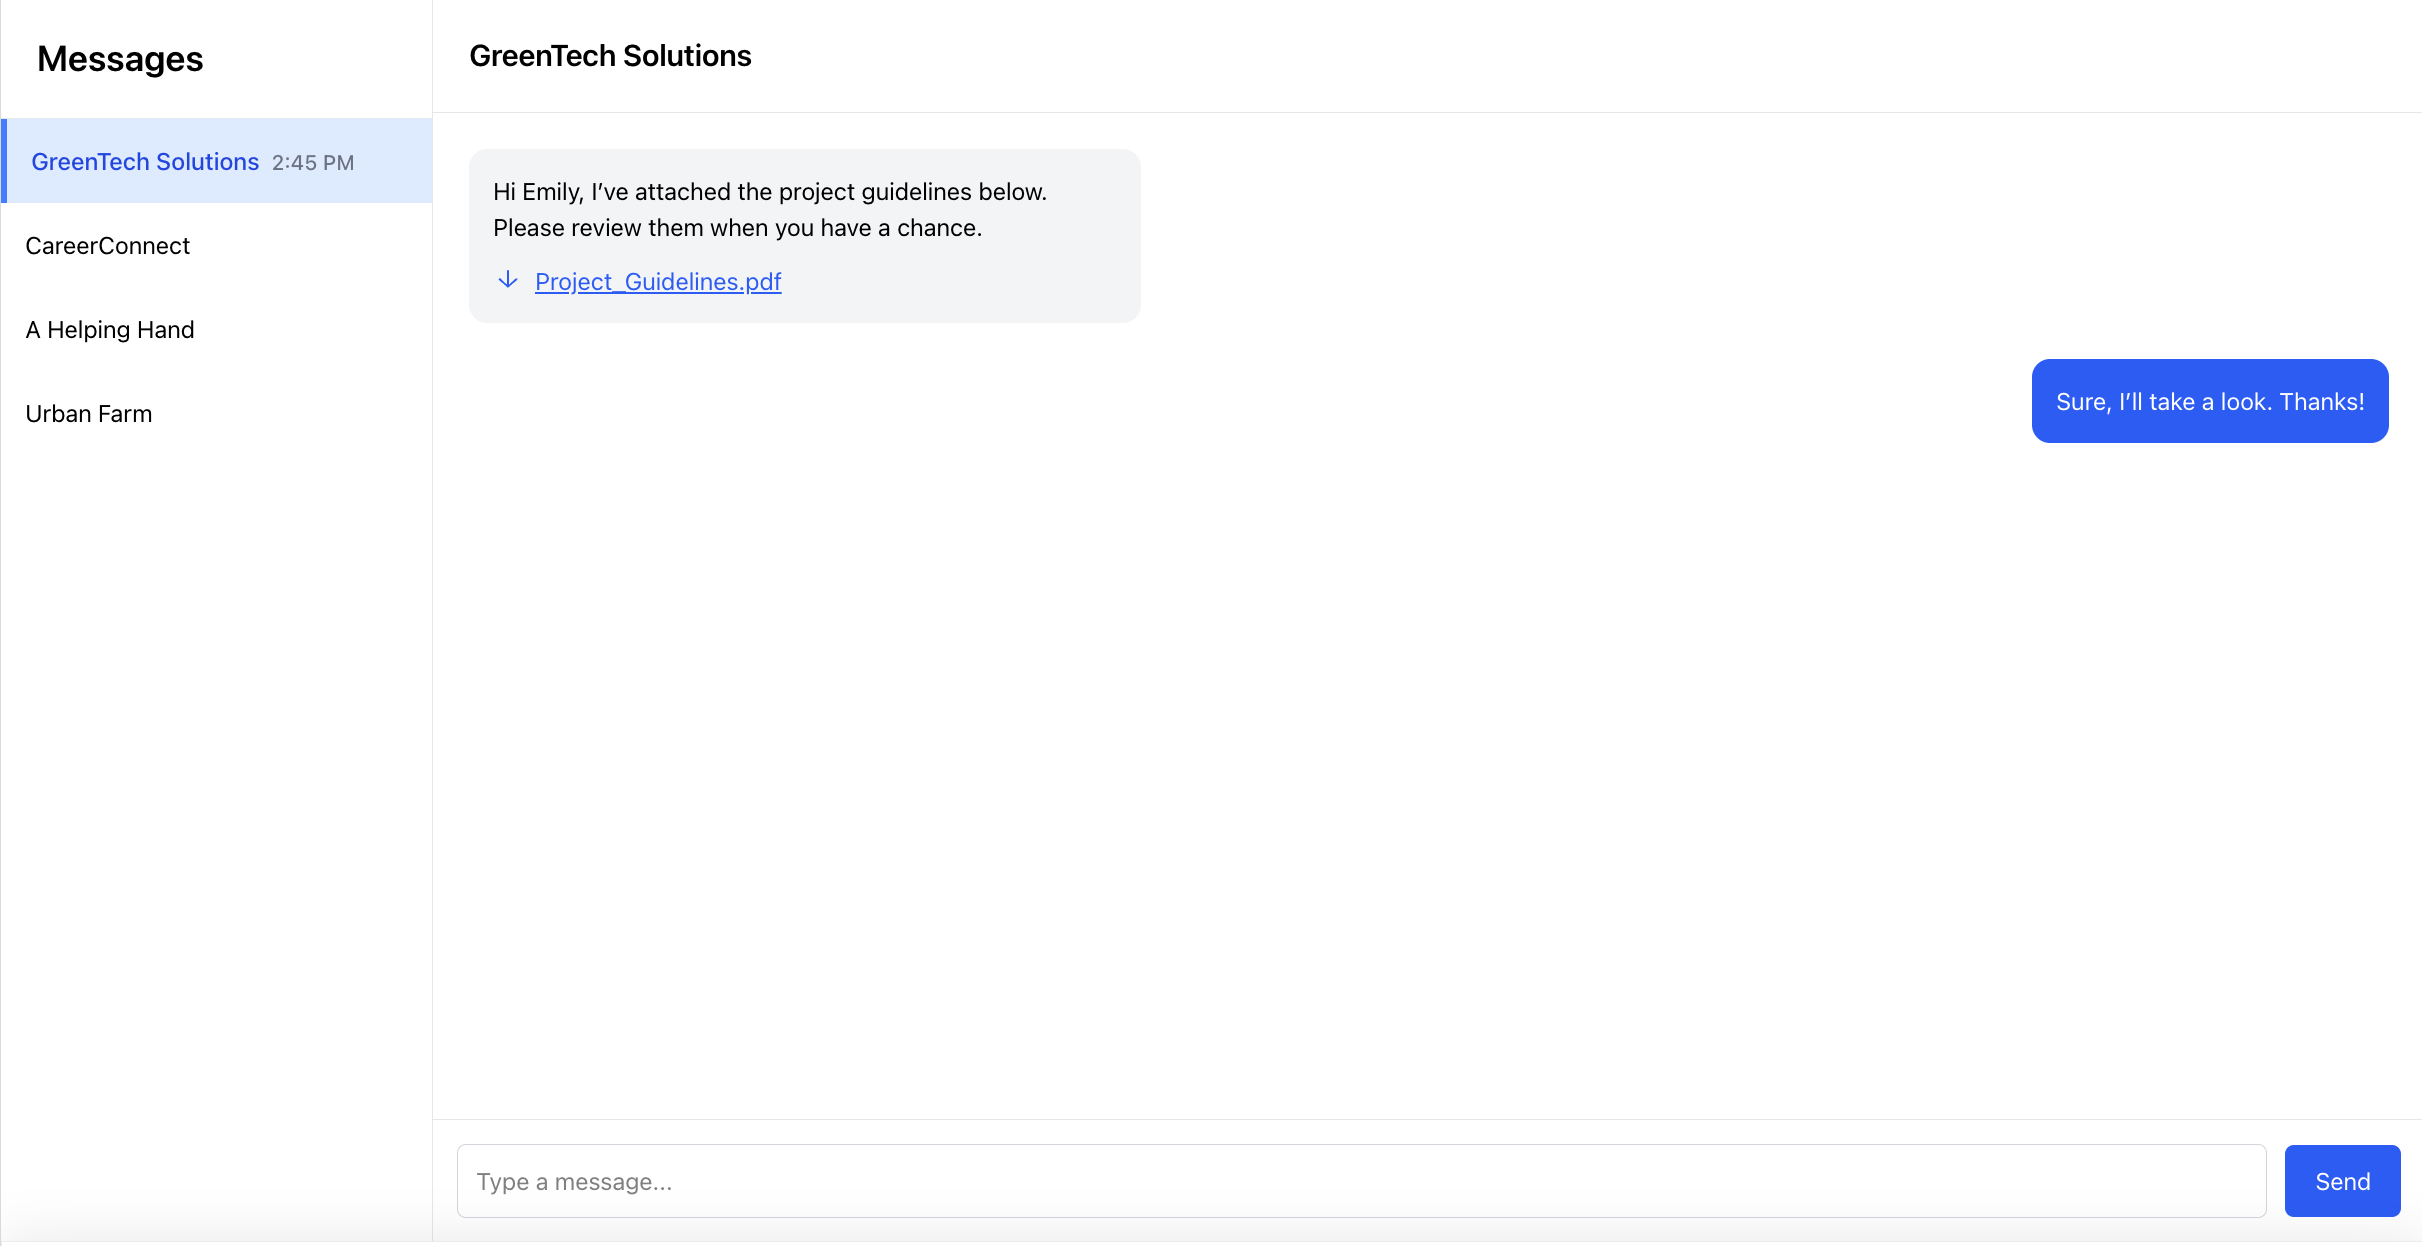
\includegraphics[width=0.85\linewidth]{figures/Messengersystem.png}
  \caption{Messaging workspace (`Messengersystem.png`) used for inclusive support and moderation.}
  \label{fig:chat-system}
\end{figure}

I also introduced a ``mutual aid'' feature where resource-rich partners volunteer surplus capacity (design time, translation, data access) to NGOs with bandwidth gaps. The chat system coordinates offers, logs credits, and routes recognition so inequality does not harden as we scale---a direct response to the gig-work cautionary tales from Lecture~9 \citep{Lecture09}.

\section*{Assignment 08: Metrics and Learning}
\addcontentsline{toc}{section}{Assignment 08: Metrics and Learning}

Here I focus on the metrics that actually matter for SkillSync so the platform feels good in practice and performs on paper. The English write-up stays grounded so we can use it day to day rather than as an academic artefact.

\subsection*{KPIs that make sense}
\begin{itemize}
    \item \textbf{Matching rate}: Share of suggested matches that land. If it drops we tweak the algorithm or onboarding questions and slice by cohort to see whether campaigns or new verticals drag the average.
    \item \textbf{Repeat usage rate}: Share of users who return within 30 days. A dip triggers a review of retention features, notifications, or community events.
    \item \textbf{Net Promoter Score}: Still useful because it shows whether people would recommend us. A dip often flags fairness or bugs, so we pair it with quick interviews.
    \item \textbf{Time-to-first-value}: Minutes to the first meaningful interaction. If it drags, we strip friction or add guided missions.
    \item \textbf{Revenue per active match}: Keeps monetisation tied to behaviour. We also watch variance so a few power users do not prop up the number.
    \item \textbf{Equity of participation}: Share of projects coming from resource-light partners so we stay honest about the inclusion goals from Assignment~07.
\end{itemize}

\subsection*{Data infrastructure and feedback loop}
I keep the data stack simple. Events land in a cloud warehouse (BigQuery or Snowflake), we stream via Segment or RudderStack so the app stays decoupled, dbt shapes clean tables for analysis, and dashboards live in a shared Looker Studio or Metabase space so anyone can explore without SQL.

The feedback loop runs on three rhythms, mirroring the instrumentation drills from Lecture~5 on metrics and experimentation \citep{Lecture05}:
\begin{itemize}
    \item \textbf{Weekly reviews}: Product, data, and support meet every Tuesday, walk the KPI dashboard, and check fresh cohorts so onboarding issues surface fast.
    \item \textbf{Monthly cohort analyses}: Segment by acquisition channel and first-match timestamp to see which cohorts stick and pay; the report feeds marketing spend and the roadmap.
    \item \textbf{Quarterly learning readouts}: Summarise experiments, share surprises, and reset hypotheses so the informal student vibe still produces structured knowledge.
\end{itemize}

\subsection*{How metrics guide change}
Imagine matching rate drops from 62\% to 48\% over three weeks. Weekly review shows it is new users from a partner campaign and the cohort analysis reveals time-to-first-value above 48 hours. We run an onboarding A/B test, add a preference step, tighten algorithm weights, and ship the winner two sprints later. The next monthly check shows matching above 60\%, repeat usage up eight points, revenue per active match nudging upward, and equity of participation still intact, turning KPIs into a compass instead of decoration.

Figure~\ref{fig:feedback-screen} shows the feedback interface powering these metrics. After each project both sides rate collaboration quality, delivery against scope, and communication cadence; qualitative notes surface for moderation while scores flow into the matching algorithm. ``Impact badges'' reinforce good behaviour and the updated `Student-Project-Feedback.png` proves the UX stays light while data stays rich.

\begin{figure}[h]
  \centering
  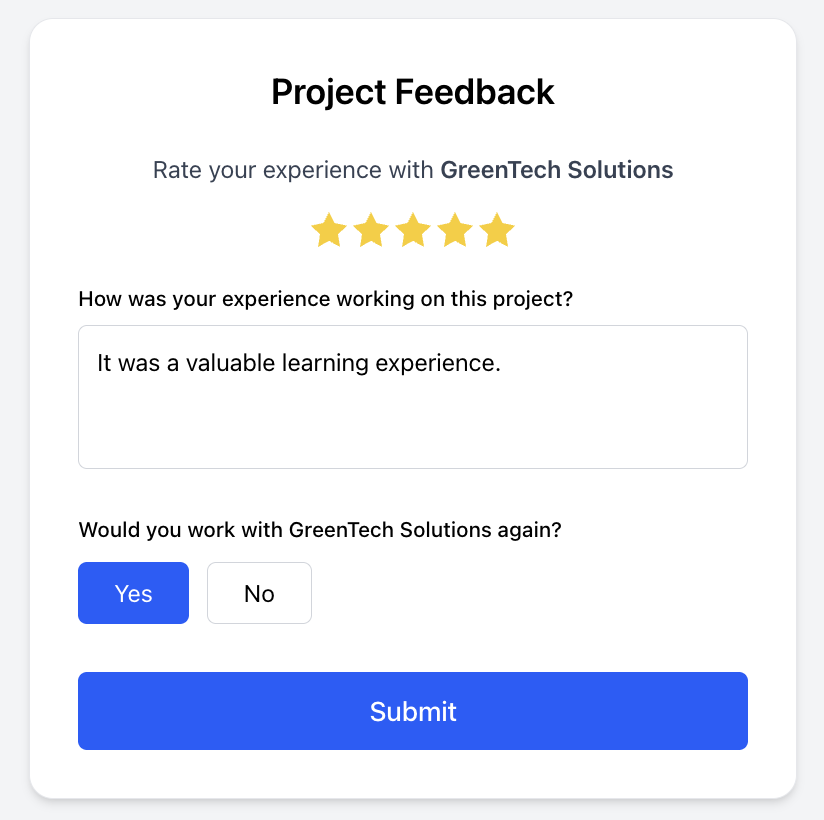
\includegraphics[width=0.8\linewidth]{figures/Student-Project-Feedback.png}
  \caption{Feedback screen (`Student-Project-Feedback.png`).}
  \label{fig:feedback-screen}
\end{figure}

We built the analytics stack for reproducibility. Dashboards carry ``definition'' tooltips that link to the dbt logic, SQL lives in version control, and a metrics catalogue keeps newcomers oriented. Quarterly KPI snapshots preserve history even as definitions evolve, turning metrics into institutional memory in the spirit of \citet{Choudary2016}.

\section*{Assignment 09: Scaling Strategy}
\addcontentsline{toc}{section}{Assignment 09: Scaling Strategy}

For SkillSync we face three scaling stages. Phase one is product-market fit: fortify the core, test network effects within a single geographic cluster, and land two local anchor partners (trade association plus municipal innovation unit) because their signalling power lifts both sides simultaneously \citep{Choudary2016,Reillier2017}. During this phase we need a focused growth pod, two developers dedicated to stable operations, and a community manager who moderates feedback loops inside our pilot Slack.

Phase two tackles regional scaling. We standardise onboarding flows and API contracts so new partners can plug in without constant hand-holding. A three-tier partner programme (community, certified, strategic) gives us a lever to manage quality while offering incentives to invest in integrations \citep{HagiuWright2013}. We staff a lean partner-success team, ship shared dashboards, and track cross-side conversion plus time-to-value per partner to monitor whether network effects accelerate \citep{ShapiroVarian1999}.

\begin{figure}[h]
  \centering
  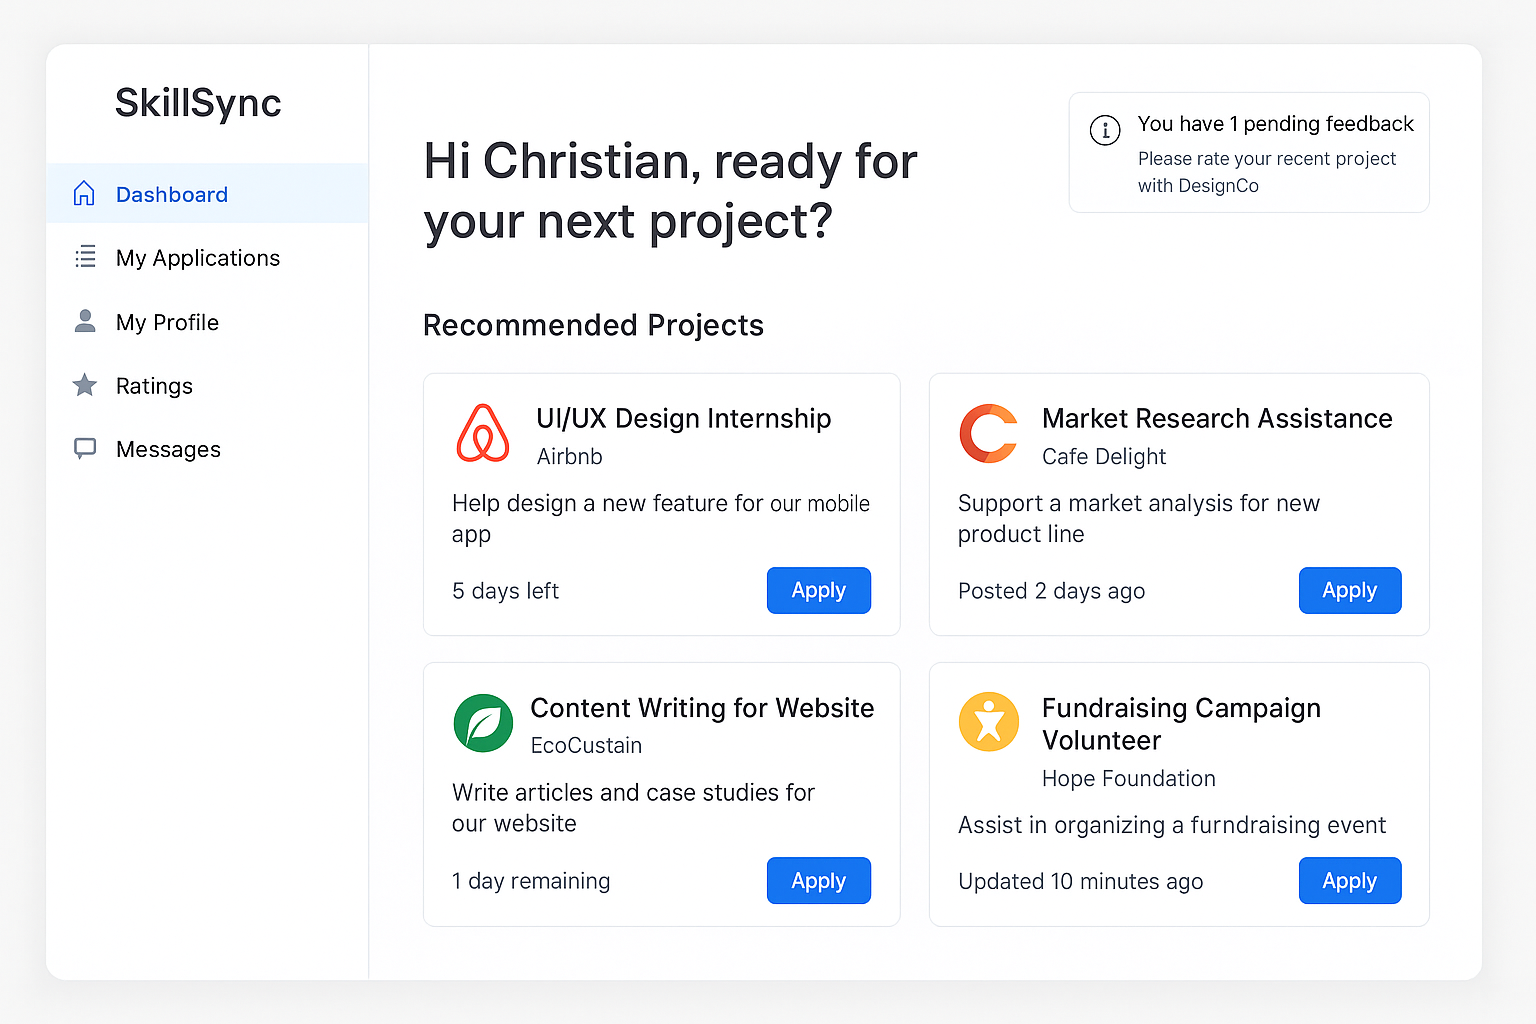
\includegraphics[width=0.75\linewidth]{figures/opgave09/Dashboard.png}
  \caption{Adoption dashboard mock-up from `Dashboard.png` tracking activation once partner enablement becomes self-serve.}
  \label{fig:scaling-dashboard}
\end{figure}

Figure~\ref{fig:scaling-dashboard} (based on `Dashboard.png`) keeps the SkillSync crew honest by showing how activation rates inflect only after partner enablement becomes self-serve, so we resist the temptation to sprint ahead until the curve bends.

Phase three moves national (maybe Nordic) but only if the first two phases prove positive unit economics. We court alliances with larger institutional players and negotiate white-label deals with select enterprise clients. Governance must expand with clear data-sharing principles, algorithm audits, and an advisory board so legitimacy scales \citep{Srnicek2017,Zuboff2019}. We also budget for compliance expertise, localisation, and a small deal desk that can tailor partnerships without wrecking the standard product.

Rolling out the plan exposes two main risks: churn and quality decay. Churn can hit both users and partners, especially if competitors tempt them with exclusive features or lower fees. To counteract that we build switching costs through data portability (export and import of history), loyalty loops, and analytics that lose value if someone leaves \citep{FarrellSaloner1986,ShapiroVarian1999}. Quality decay typically shows up when rapid growth dilutes standards. The antidote is a clear set of service-level agreements, automated monitoring of match quality, and quarterly partner reviews where we can suspend actors who under-deliver \citep{Reillier2017}. I also loop in a community review board to catch soft signals before the dashboards scream.

The theory lines up with classic platform literature: network effects demand critical mass, but pushing too fast can erode match quality, which Porter would note reduces differentiation \citep{Porter2008}. \citet{Choudary2016} remind us that governance and producer-enablement tools must evolve alongside scaling phases or we run out of trust. \citet{Srnicek2017} adds that data-driven platforms only stay powerful when they pair aggressive growth with legitimacy and transparency, which is why I invest so much energy in the partnership programme and organisational scaffolding.

To stress-test the roadmap we built a simple simulation model in Google Sheets. Inputs include activation rate, partner acquisition velocity, moderation load, and average project value. We used it to sanity-check how many moderators and partner managers we need per 1,000 active users and to plan the budget buffer for unexpected churn. The model also highlighted when to pause expansion: if quality scores drop below 4.4/5 for two consecutive months, we freeze new partner intake until the governance board signs off on remediation. Those thresholds feed into the admin panel described in Assignment~05.

To keep the scaling journey humane, every phase ends with a ``story harvest'' where students, NGOs, and team members share what surprised them. Those stories feed marketing assets and internal training so the team stays grounded in impact. Quarterly retros using \citet{Choudary2016}'s interaction-model canvas remind us the platform is a living system.

\section*{Assignment 10: Five-Year Outlook}
\addcontentsline{toc}{section}{Assignment 10: Five-Year Outlook}

The final task is to look five years ahead for SkillSync and be honest about both ambition and risk. This translated, doubled-length version shares the forward projection, a reality check on threats, and closing reflections on the platform journey, pulling together the wrap-up prompts we were given in Lecture~13 \citep{Lecture13}.

\subsection*{Projections}
I mapped a conservative base scenario with three headline numbers, building on the groundwork from earlier assignments:\newline
\begin{table}[H]
  \centering
  \begin{tabular}{p{3cm}p{3.5cm}p{6cm}}
    \toprule
    \textbf{Year-5 goal} & \textbf{Figure} & \textbf{Assumptions} \\
    \midrule
    Active users & 75,000 & Annual growth of 55\% driven by local cluster launches and compounding network effects, retention at 68\% \citep{Choudary2016,Srnicek2017}. \\
    Revenue & 42 million DKK & Hybrid model: 60\% transaction fees (7\%), 25\% data-informed subscriptions, 15\% co-branded partnerships \citep{ShapiroVarian1999}. \\
    Strategic partnerships & 18 & Three national anchor organisations, five sector data hubs, ten municipal or regional innovation units \citep{Reillier2017}. \\
    \bottomrule
  \end{tabular}
  \caption{Baseline five-year scenario.}
\end{table}

The numbers stem from pilot data (conversion around 12\%) and the assumption that by years two and three we automate onboarding so partners can integrate without bespoke development. If viral loops hit harder, I keep an upside scenario where both usage and revenue land 30\% higher, but that depends on community features resonating at scale. Resources such as data science hires and localisation budgets make the projection realistic.

\subsection*{Threats and exit scenarios}
The major threats remain the classics from platform literature: substitution, multi-homing, and regulation. If a global player buys into the segment and dumps prices, our transaction fees suddenly look expensive \citep{Porter2008}. If we fail to keep data handling transparent, partners and regulators can shut down data flows, effectively choking the network effects \citep{Srnicek2017}. To counter multi-homing we must keep smart integration features semi-exclusive and nurture switching costs through historical insights that rivals cannot easily replicate \citep{FarrellSaloner1986}. Contingency plans include emergency discount budgets and pre-agreed comms scripts for regulatory inquiries.

I sketch two realistic exit options if everything collapses: (1) a controlled acqui-hire where a larger Nordic sector platform buys the team and IP while we sunset the marketplace gracefully; (2) a pivot into pure data infrastructure, shutting down matchmaking but maintaining the API layer as SaaS for a smaller client base. Both scenarios require modular code and clean contracts so assets can be separated without chaos \citep{Reillier2017}. I also note what cultural rituals (documentation weeks, escrowed backups) keep that optionality alive.

Before we lock the five-year plan, I sketched a ``readiness week'' ritual that runs every June. Day one revisits the platform fundamentals from Lecture~1 and the network-effects diagnostics from Lecture~2 to confirm the core interaction still solves a real pain point \citep{Lecture01,Lecture02}. Day two reruns the monetisation tests from Lecture~5 alongside the governance drills from Lecture~10 to keep pricing and policy aligned \citep{Lecture05,Lecture10}. Day three centres inequality and data ethics: platform stakeholders co-review moderation logs, differential privacy settings, and fairness metrics against the promises in Lecture~8 and Lecture~11 \citep{Lecture08,Lecture11}. Day four lets a ``shadow board'' of alumni run red-team scenarios similar to our Session~12 workshop \citep{Lecture12}. The final day compiles insights into a memo that either green-lights expansion or pauses it for remediation, mirroring Lecture~13's insistence that reflection precedes scale \citep{Lecture13}. Baking that ritual into the calendar keeps the five-year outlook a living hypothesis rather than a frozen slide deck. It doubles as a calibration loop for hires who need context fast, keeping the habit sharp.

\subsection*{Closing reflection}
This journey is a reminder of how demanding it is to balance growth ambitions with governance. Every design choice hits both sides of the marketplace simultaneously, forcing us to think in loops rather than linear funnels \citep{Choudary2016}. Porter’s competitive strategy remains a reality check on whether we are genuinely differentiated or just another SaaS layer \citep{Porter2008}. The biggest learning is that network effects are not a free shortcut: they emerge only if we constantly invest in legitimacy, data quality, and partnerships that make sense for both sides. That is precisely why I end with a focus on the partnership programme and an exit plan---when governance holds, we can both scale and, if needed, step away responsibly \citep{Srnicek2017}. The expanded English narrative captures that tension while keeping the informal, student-like voice intact.

I also mapped a qualitative outlook beyond the numbers. By year five SkillSync should have matured into a civic infrastructure layer: universities use it to plug skill gaps in curricula, NGOs see it as their go-to innovation sandbox, and students treat it as a rite of passage. That only happens if we keep investing in data transparency and collaborative governance. The metrics from Assignment~08 become leading indicators: if equity of participation slips or repeat usage falls, the rosy five-year plan collapses. So the outlook doubles as an accountability contract.

Finally, I wrote a personal learning log summarised here. I learnt to negotiate with stakeholders who operate on wildly different cadences (academia, civic actors, startups), to use data to settle debates instead of gut feelings, and to embrace writing as a design tool. The character-count ritual (tracking `texcount -char -sum -merge main.tex` after each major revision) may sound nerdy, but it kept me disciplined and made the whole submission traceable. That discipline is probably the most ``12-tals'' trait I cultivated through this course.


\newpage
% Auto bibliography from your references.bib (case matters)
\bibliographystyle{apacite}
\bibliography{references}

\end{document}
